Our solar system was formed 4.5 billion years ago, when about $2\%$ of the galaxy's original Hydrogen and Helium had been converted to heavier elements. Thus the cloud which formed our galaxy was roughly $98\%$ Hydrogen and Helium. The $2\%$ of other materials form the core of the rocky planets in our systems, ie. the Earth.

The {\bf Andromeda galaxy} is roughly 2.5 million light-years away and about $100,000$ light-years in diameter. {\bf Sirius}, the brightest star visible in the night sky, is 8 light-years away. {\bf Alpha Centauri}, the closest star system to our own (a three star system), is 4.4 light-years away.

\begin{itemize}
\item $E_k = \frac{1}{2}mv^2$
\item $v = \lambda f$
\item $\text{Energy} = h f = \frac{hc}{\lambda}$
\item $v_\text{radial} = \frac{\Delta \lambda}{\lambda}\ c$
\item $F = G\frac{m_1 m_2}{r^2}$
\item $p^2 = \frac{4\pi^2}{(M_1 + M_2) * G}\ a^3$ (in our solar system $\text{years}^2 = \text{A.U.}^3$)
\item $L = 4\pi^2R^2 \sigma_{SB} T^4$
\item Angular separation (rad) $= \frac{\text{semi-major axis (AU)}}{\text{distance parsecs}}$
\item $r_\text{planet} \approx r_\text{star} * \sqrt{\text{fraction of light blocked}}$
\item Eccentricity of an ellipse: $e = \frac{f}{a}$ where f is the distance from the center to a focus
\item $\text{momentum} = \text{mass} * \text{velocity}$
\item $\text{SA}_\text{sphere} = 4 \pi r^2$
\item $\lambda_\text{peak} T = 2.898 * 10^{-3} m \cdot K$
\item Time dilation: $t' = t * \sqrt{1 - \left( \frac{v}{c} \right)^2}$
\item Length contraction: $l' = l * \sqrt{1 - \left( \frac{v}{c} \right)^2}$
\item Mass increase: $m' = \dfrac{m}{\sqrt{1 - \left( \frac{v}{c} \right)^2}}$
\item Angular size, physical size, and distance are related as $\frac{l_{angular}}{360} = \frac{l_{physical}}{2\pi d}$
\item $v = \sqrt{\frac{M_r * G}{r}}$
\begin{itemize}
    \item $M_r$ = encircled mass
    \item $r$ = radius of sphere containing the mass
\end{itemize}
\end{itemize}


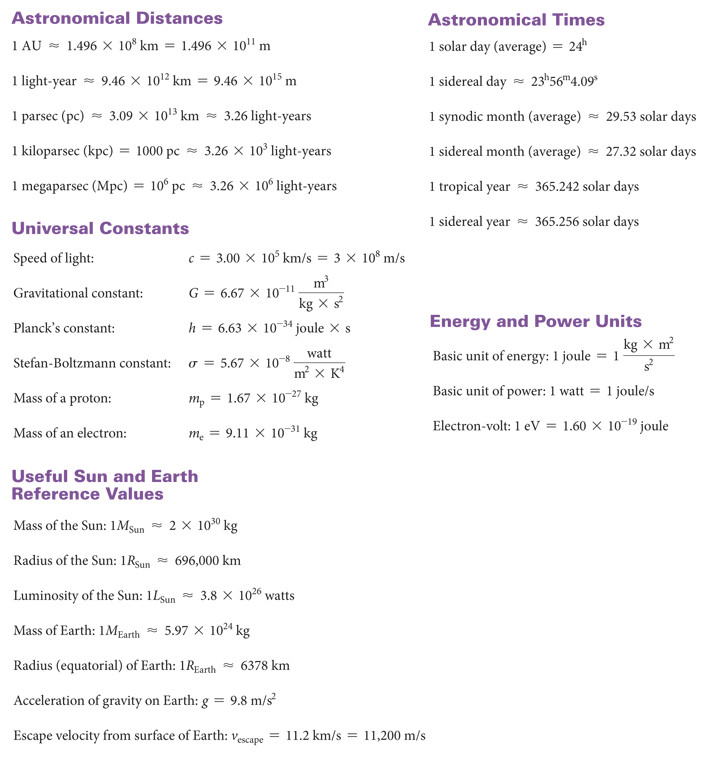
\includegraphics[width=\textwidth]{constants}
